\chapter{Introduction}

Previous large scale surveys of galaxies have revealed a bimodality in the colour-magnitude diagram (CMD) with two distinct populations; one at relatively low mass, with blue optical colours and another at relatively high mass, with red optical colours \citep{Baldry04, Baldry06, Willmer06, ball08, Brammer09}. These populations were dubbed the `blue cloud' and `red sequence' respectively \citep{Chester64, bower92, Driver06, Faber07}. The Galaxy Zoo project \citep{Lintott11}, which produced morphological classifications for a million galaxies, helped to confirm that this bimodality is not entirely morphology driven \citep{Strat01, Salim07, Sch07, CHV08, Bamford09, Skibba09}, detecting larger fractions of spiral galaxies in the red sequence \citep{masters10c} and elliptical galaxies in the blue cloud \citep{Sch09} than had previously been detected.

The sparsely populated colour space between these two populations, the so-called `green valley', provides clues to the nature and duration of galaxies' transitions from blue to red. This transition must occur on rapid timescales, otherwise there would be an accumulation of galaxies residing in the green valley, rather than an accumulation in the red sequence as is observed \citep{Arnouts07, Martin07}. Green valley galaxies have therefore long been thought of as the `crossroads' of galaxy evolution, a transition population between the two main galactic stages of the star forming blue cloud and the `dead' red sequence \citep{Bell04, Wyder07, Schim07, Martin07, Faber07, Mendez11, Gonc12, schawinski14, Pan14}. 


The intermediate colours of these green valley galaxies have been interpreted as evidence for recent quenching (suppression) of star formation \citep{Salim07}. Star forming galaxies are observed to lie on a well defined mass-SFR relation, however quenching a galaxy causes it to depart from this relation (\citealt{Noeske07, peng10}).


By studying the galaxies which  have just left this mass-SFR relation, I can probe the quenching mechanisms by which this occurs. There have been many previous theories for the initial triggers of these quenching mechanisms, including negative feedback from AGN \citep{diMatteo05, Martin07, Nandra07, Sch07}, mergers \citep{Darg10a, Cheung12, Barro13}, supernovae winds \citep{MFB12}, cluster interactions \citep{Coil08, Mendez11, Fang13} and secular evolution \citep{masters10c, masters11a, Mendez11}. By investigating the \emph{amount} of quenching that has occurred in the blue cloud, green valley and red sequence; and by comparing the amount across these three populations, I can apply some constraints to these theories. 


The nature of the observed co-evolution of galaxies and their central supermassive black holes \citep{magorrian98, marconi03, haringrix04} and the effects of AGN feedback on galaxies are two of the most important open issues in galaxy evolution. AGN feedback was first suggested as a mechanism for regulating star formation in simulations \citep{silk98, Croton06, Bower06, somerville08} and indirect evidence has been observed for both positive and negative feedback in various systems (see the comprehensive review from \citealt{fabian12}). 

The strongest observational evidence for AGN feedback in a population is that the largest fraction of AGN are found in the green valley \citep{cowie08, Hickox09, schawinski10a}, suggesting some link between AGN activity and  the process of quenching which moves a galaxy from the blue cloud to the red sequence. However, concrete statistical evidence for the effect of AGN feedback on the host galaxy population has so far been elusive.

There are many mechanisms which are proposed to cause quenching; including mergers \citep{daddi10}, mass quenching \citep{kennicutt87, peng12}, morphological quenching \citep{?} and the environment of a galaxy.
 
 The galaxy environment as a cause of quenching was proposed due to the correlation of both morphology \citep{dressler80} and the quenched galaxy fraction \citep{?} with environmental density. 
 
 BUT does this correlation truly imply causation? Evidence from simulations \citep{?} suggests that the environment may not be the dominant quenching mechanisms for galaxies. Perhaps the correlation of increased galaxy quenched fractions with environment is due to a combination of mergers, mass and morphological quenching. In denser environments, galaxies are more likely to encounter another galaxy in a merger scenario and large viral radii give rise to long infall times during which gas reservoirs can be depleted due to star formation.
 
 To study this I need to look at how quenching timescale changes in groups and clusters of galaxies with different properties in order to isolate the cause of the density-morphology and density-SFR correlations. 

\section{Galaxy Zoo}

In this investigation I use visual classifications of galaxy morphologies from the Galaxy Zoo 2\footnote{\url{http://zoo2.galaxyzoo.org/}} citizen science project \citep{GZ2}, which obtains multiple independent classifications for each galaxy image; the full question tree for each image is shown in Figure 1 of \citealt{GZ2}.  

The Galaxy Zoo 2 (GZ2) project consists of $304, 022$ images from the SDSS DR8 (a subset of those classified in Galaxy Zoo 1; GZ1) all classified by \emph{at least} 17 independent users, with the mean number of classifications standing at $\sim42$. The GZ2 sample is more robust than the GZ1 sample and provides more detailed morphological classifications, including features such as bars, the number of spiral arms and the ellipticity of smooth galaxies. It is for these reasons I use the GZ2 sample, as opposed to the GZ1, allowing for further investigation of specific galaxy classes in the future (see Section~\ref{future}). The only selection that was made on the sample was to remove objects considered to be stars, artefacts or merging pairs by the users (i.e. with $p_{star/artefact} ~\geq~ 0.8$ or $p_{merger} ~\geq 0.420$; see \citealt{GZ2} Table 3 and discussion for details of this fractional limit). Further to this, I required NUV photometry from the GALEX survey, within which $\sim42\%$ of the GZ2 sample were observed, giving a total sample size of $126, 316$ galaxies. The completeness of this subsample of GZ2 matched to GALEX is shown in Figure~\ref{complete} with the $u$-band absolute magnitude against redshift for this sample compared with the SDSS data set. Typical Milky Way $L_*$ galaxies with $M_u \sim -20.5$ are still included in the GZ2 subsample out to the highest redshift of $z \sim 0.25$; however dwarf and lower mass galaxies are only detected at the lowest redshifts.

The first task of GZ2 asks users to choose whether a galaxy is mostly smooth, is featured and/or has a disc or is a star/artefact. Unlike other tasks further down in the decision tree, every user who classifies a galaxy image will complete this task (others, such as whether the galaxy has a bar, is dependent on a user having first classified it as a featured galaxy). Therefore I have the most statistically robust classifications at this level.

The classifications from users produces a vote fraction for each galaxy (the debiased fractions calculated by \citet{GZ2} were used in this investigation); for example if 80 of 100 people thought a galaxy was disc shaped, whereas 20 out of 100 people thought the same galaxy was smooth in shape (i.e. elliptical), that galaxy would have vote fractions $p_{s} = 0.2$ and $p_{d} = 0.8$. In this example this galaxy would be included in the \emph{`clean'} disc sample ($p_d \geq 0.8$) according to \cite{GZ2} and would be considered a late-type galaxy. All previous Galaxy Zoo projects have incorporated extensive analysis of volunteer classifications to measure classification accuracy and bias, and compute user weightings (for a detailed description of debiasing and consistency-based user weightings, see either Section 3 of \citealt{Lintott09} or Section 3 of \citealt{GZ2}). 

\begin{figure*}
\centering{
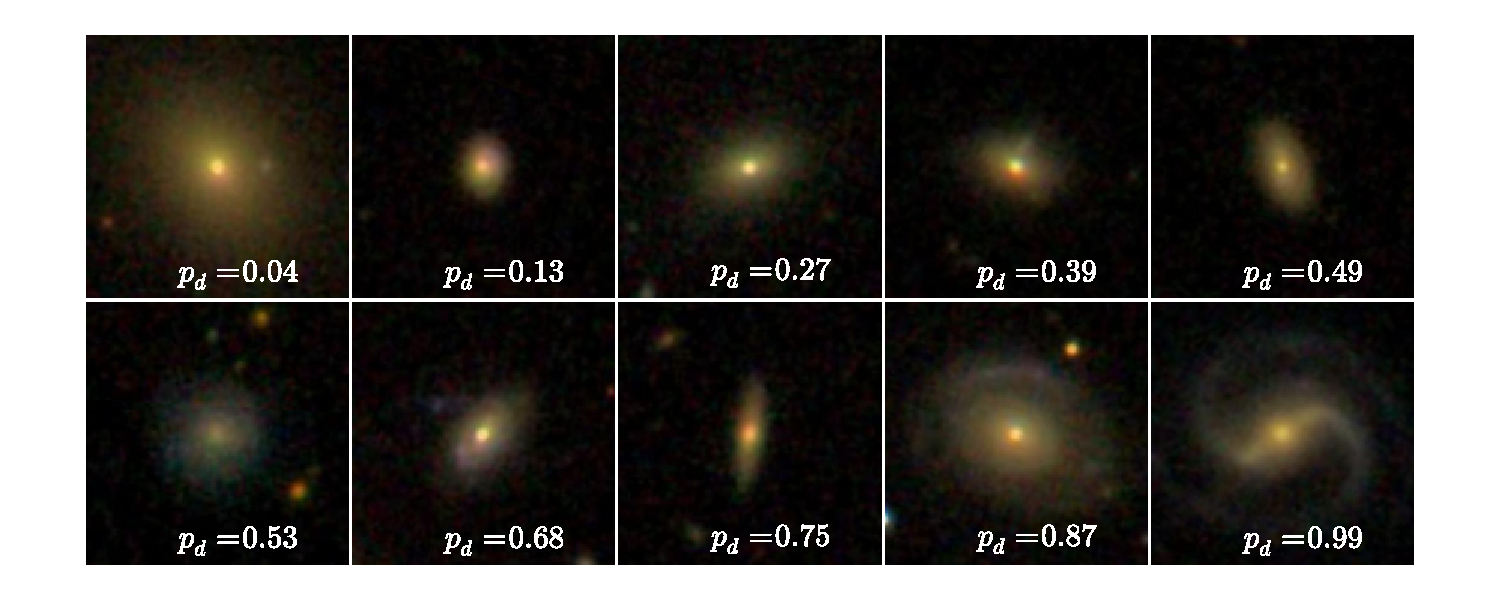
\includegraphics[width=\textwidth]{introduction/mosaic_disc_fraction_z_0-07_0-075.pdf}}
\caption[Example SDSS images with GZ2 vote fractions]{Randomly selected SDSS \emph{gri} composite images showing the continuous probabilistic nature of the Galaxy Zoo sample from a redshift range $0.070 < z < 0.075$. The debiased disc vote fraction (see \citealt{GZ2}) for each galaxy is shown. The scale for each image is $0.099~\rm{arcsec/pixel}$.}
\label{mosaic}
\end{figure*}

The classifications are highly accurate and provide a continuous scale of morphological features, as shown in Figure~\ref{mosaic}, rather than a simple binary classification separating elliptical and disc galaxies. These classifications allow each galaxy to be considered as a probabilistic object with both bulge and disc components. 
